% Experiments

This section presents the experiments and results aimed at evaluating our proposed graph generative model. First we run a grid-search on the hyperparameter space to find the optimal configuration of the RGVAE. We use the ELBO and MRR as evaluation metric. The best configurations are used to perform link prediction. Here we compare the model performance with vs. without convolutions. We use the VDistMult as control model for link prediction. Finally we run two proof-of-concept experiments. The first generating triples and filter on a entity class constraining relation, thus we get an insight of how much percent of the generated triples are valid. Secondly we analyze the results of a RGVAE trained on subgraphs with $n=10$. For the experiments we use two multi-relational KG datasets.

% We covered link and node prediction and compared those to SOTA scores. Further we ran experiments on investigating the coherence of the reproduced graph structure. Lastly we measured the adherence of our model to the KG's underlying syntax.


\subsection{Data}
For this sake of comparison with state of the art results, we chose the two most popular dataset used in this field of KG link prediction, FB15k237 and WN18rr.

% Training models on each dataset for 333 epochs, without early stopping.

\textbf{Fb15k-237}

\printinunitsof{in}\prntlen{\textwidth}

Entity types

triple topics

This dataset is a subset of the FreeBase KG (cite).[Explain Free Base] The original Fb15k had redundant triples, creating ambiguity during training. In the updated version, Fb15k-237, these triples were removed what led to a more robust dataset, which is commonly used as benchmark for several NLP tasks.

% or/and
A subset from one of the first and largest KGs, called FreeBase. In the first version of this dataset, it was possible to infer most of the test triples by inverting triples in the trainset, Thus the latest $237$ version filtered these triples out.
The dataset contains $14,951$ entities and $1,345$ different relations.

\textbf{WN18rr}

Based on the wordnet KG.

% Table comparing numbers

\subsection{Hyperparameter Tuning}

In this section we run a grid search for the three hyperparameters $\beta$, $d_z$ and $d_h$ for a set of contrastive values. To reduce the computational expenses we train each model for $60$ epochs and  evaluate link prediction on a subset of $50$ triples.

Empirically we set the learning rate to $3e-5$ and the batchsize to the maximum fir on the GPU memory. For $d_h$ we did not see any significant changes for higher values, thus we choose a lower number to reduce the total model parameters. The remaining hyperparameter did influence and the optimal setting vary for each dataset, table \Ref shows the results of our hyperparameter tuning.

% lr empirically and batchszize fixed.

% beta
For the hyperparameter tuning of $\beta \in [0,1,10,100]$ we chose significant values. With $\beta = 0$ we do not constrain our model on the Gaussian prior, thus the latent distribution can take the form of any distribution. This reduces the influence of the variational module and the model becomes closer to an autoencoder. For $\beta = 1$ we get our base model, and for $\beta \in [10,100]$ the $\beta-$VAE version.


\begin{figure}[H]
    \centering
    \begin{subfigure}{.5\textwidth}
      \centering
      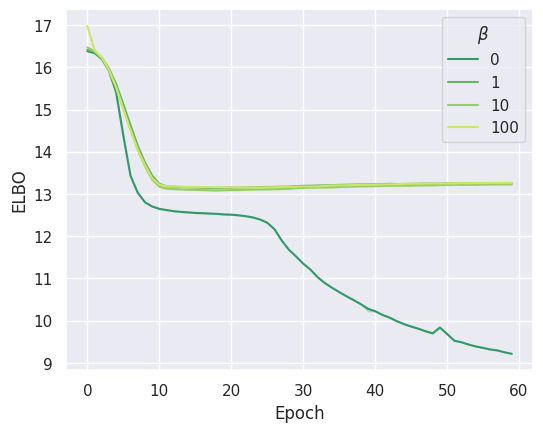
\includegraphics[width=.9\linewidth]{graphs/plots/beta_loss_fb.png}
      \caption{FB15K-237}
      \label{fig5:betafb}
    \end{subfigure}%
    \begin{subfigure}{.5\textwidth}
      \centering
      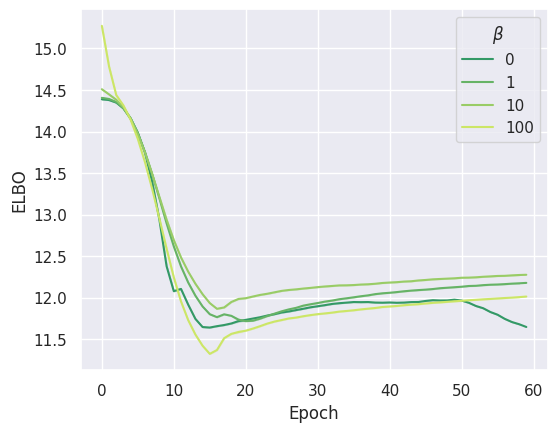
\includegraphics[width=.9\linewidth]{graphs/plots/beta_loss_wn.png}
      \caption{WN18RR}
      \label{fig5:betawn}
    \end{subfigure}
    \caption{Validation loss for RGVAE with $\beta \in [0,1,10,100]$ trained on each dataset.}
    \label{fig5:beta}
\end{figure}


Figure \ref{fig5:beta} shows the validation ELBO for the different $\beta$ values and for both datasets. We notice two interesting outcomes.  

\begin{enumerate}
    \item For $\beta = 0$ converges further than the rest.
    \item The remaining values behave quase identical with $\beta = 100$ performing slightly better. 
\end{enumerate}

Since setting $\beta = 0$ would undermine our hypothesis of evaluating variational model, we chose $\beta = 100$ as default for the following experiments. This also compares with the $\beta$ values proposed by Higgins in \cite{higgins_beta-vae_2016} to achive a factorization of the latent space.

Especially on the FB15k-237 dataset the $\beta = 0$ configuration converges to a much lower ELBO. Thus, we have the trained models perform link-prediction on a $1\%$ subset of the validation set. The barplot \ref{fig5:betafbmrr} indicates an inverse correlation between the ELBO and the MRR score. 

\begin{figure}[H]
    \centering
      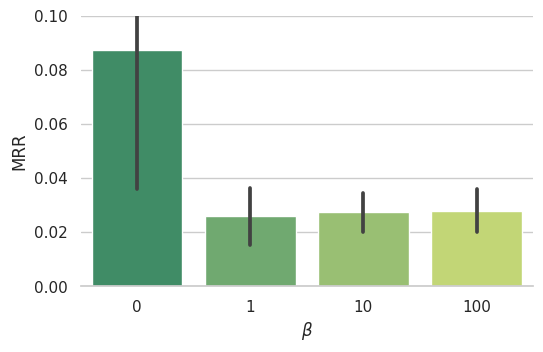
\includegraphics[width=.45\textwidth]{graphs/plots/beta_mrr_fb.png}
      \caption{MRR scores for different $\beta$ values on the dataset FB15k-237.}
      \label{fig5:betafbmrr}
\end{figure}

% d_z
Experiments on the impact of $d_z$ on the ELBO show little improvement for $10<d_z<100$ and from $100<d_z<1000$ insignificant to no improvement. Thus, we chose $d_z=100$ as default for our experiments.
TABLE IN APPENDIX  


% d_h did not influcence
Lastly, we evaluate the models hidden dimensions $d_h$ and its influence on the ELBO and the (subset)MRR. We compare between $d_h\in [256, 512, 1024, 2048]$, while the lowest configuration performs slightly worse on the ELBO, there is no significant difference the remaining three configurations. Considering the models parameter count we chose the $d_h=512$ as default.


\subsection{Link Prediction}


 We now get to the main experiment of this thesis. The results of this experiment will reveal if the RGVAE architecture is suitable for link prediction and in first palace, if it is able to grasp the underlying KG semantics at least significantly better than random by differentiating between real and corrupted triples. At this point we bring in the convolutional variation of our model, which we will denote as RGCVAE. The experiments reveal if the convolutional architecture holds an advantage compared to the simple MLP baseline. Further a randomly initiated and untrained RGVAE is used as control model.
 
 Due to its sparse graph computation, the RGVAE takes about 7 day to evaluate link prediction on the full testset and even 3 days when prediction tasks run parallel on a node of $4$ Nvidia Titan RX 25GB GPUs. Since the exemplar link prediction during experimenting with different hyperparameter already gave us an idea of the mediocre performance of our model, we chose to spare computation time and power by running link prediction on a randomly drawn one-third of the complete test set. Each run is repeated three times using a different random seed.

The results are visualized in figure \ref{fig5:lp_final}. We chose a visualization over a table, to emphasize our observations, and for the mentioned limitation of the testset, which makes these results not suitable for academic valid comparisons. Note that the figures are scales and to a range $[0,10]$ while all metrics have a maximum of $1$.

Comparing a MRR of $0.08$ to the DistMult score or $0.4$ our model does not perform competitive on link prediction tasks.
Better than random?? I hope so.

Graph convolutions do not yield and advantage over the basemodel. In fact, the RGCVAE scores even slightly worse. 

%  FOR Conclusion: this might be because of the implementation of stacking the matrices.
The model scores about three times better on the FB15k-237 dataset than on WN18RR. FB15k-237 is a richer dataset with more triples and and a more balanced ratio of entities to relations. WN18RR operates on only 18 relations, what makes the relation most crucial when completing a triple. The architecture of the RGVAE is puts twice the emphasis entities, described by the adjacency and the node feature matrices, while the relation is only represented by the overly sparse edge attribute matrix. Thus, we could conclude that our model learns to predict based on the hidden types and topics of the entities. All possible conclusions for this are discussed in \ref{sec:discus}. Relvant for this section is, that we chose the FB15k-237 dataset to investigate further, how well the RGVAE's grasps the underlying entity types and triple topics.   

%  REASON: fb has more relations, is a more complete KG. wn only 12 relations and more entities. Model emphasizes entities (adj and node features), relations may be less relevant, wn is more about the relation (same/ not the same). This indicates that our model grasps the hidden types and topics of the FB entities.


 \begin{figure}[H]
  \centering
  \begin{subfigure}{.5\textwidth}
    \left
    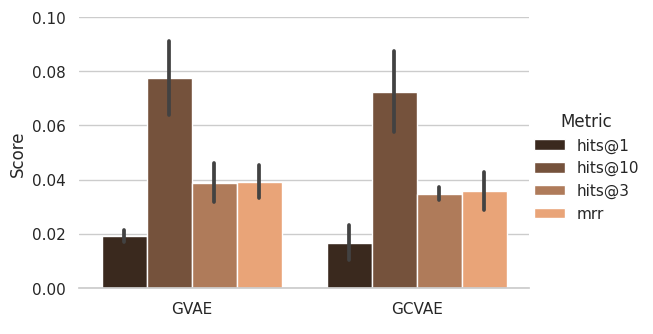
\includegraphics[height=.5\textwidth, keepaspectratio]{graphs/plots/lp_fb.png}
    \caption{FB15K-237}
    \label{fig5:lpfb}
  \end{subfigure}%
  \begin{subfigure}{.5\textwidth}
    \right
    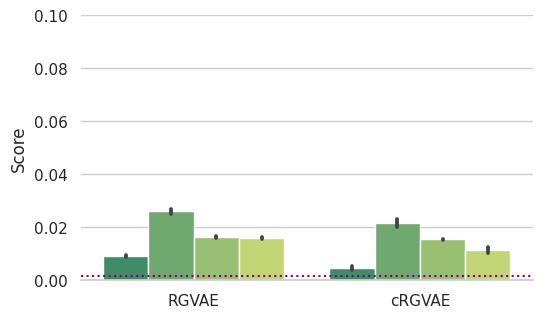
\includegraphics[height=.5\textwidth]{graphs/plots/lp_wn_wol.png}
    \caption{WN18RR}
    \label{fig5:lpwn}
  \end{subfigure}
  \caption{Link prediction results in MRR, Hits@1, Hits@3 and Hits@10 for RGVAE and RGCVAE trained on the full trainset of each dataset.}
  \label{fig5:lp_final}
\end{figure}

TODO add random!!!

% Compare with vs without convolution 
% We use negative elbo as scoring function. Since elbo is aimed to be reduced and LP scores are higher better.

% We try with and without permutation

% We try the model as encoder only NO

% We use 1/3 of the test set only, randomly drawn. Run 3 times?
% Final models only 60 epochs


\subsubsection{DistMult lp}

In order to explain the poor performance of the RGVAE on the task of link prediction, either the models architecture or the variational inference is to blame. Since the RGVAE with relaxed latent space, meaning less variance, indicated higher scorings than the Gaussian prior version, we examine the two variables by means of embedding models. The DistMult model with optimized parameter serves as control model, while we compare it to the VDistmult \ref{ssec4:vdistm} learning the full ELBO versus learning only on the reconstruction loss.



Answer question:Link prediction with control model:
Distmult vs Var Distmult vs relaxed VDistmult

We see that the variational part messes everything up.

Table:
MRR + Hits@all + Loss

\subsection{Impact of permutation}
% Check if adj matrix adheres to edge attribute matrix.

Permutation starts at 1$100\5$ at the beginning of training and converges then to $60\%$.

Model without predicts adj node always in the upper right just as the target. Model with predicts much more variations of adjacency.

Graph of permutation during training.
loss with vs without 

\subsection{Interpolate Latent Space}
We take two random triples and interpolate the latent space of these two triples. The interpolations result in: HERE AN EXAMPLE.

Further we go ahead and test what happens if we modify one latent dimension at a time with $d_z = 10$ of a triple. TABLE: (s,r,o), x_axis dims, y_axis steps. $95\%$ Gaussian confidence 

Can the model assign logical features to latent dimensions?


\subsection{Syntax coherence}

Check model trained with vs without perm invariance.

Check if generated triples follow basic logic.
\begin{itemize}
    \item Generate triples by random signals
    \item Filter these triples on type fixed relation
    \item Check if the entity is of this type.
\end{itemize}

Since there is no preset for how to check the semantics of a KG, we will use simple basic logical criteria.
The generated triples are filtered for the relation 'is capital of', thus the subject entity should be of type 'city' and the object entity of type 'country' and both adhere follow the topic 'location',
Hope this gives good results.


\subsection{Subgraph Generation}

Until now our model trained on only one triple per sparse graph. What will happen if we train it on more than one triples?
